\section{Conclusion}

\begin{figure}[H]
	\hspace{-1cm}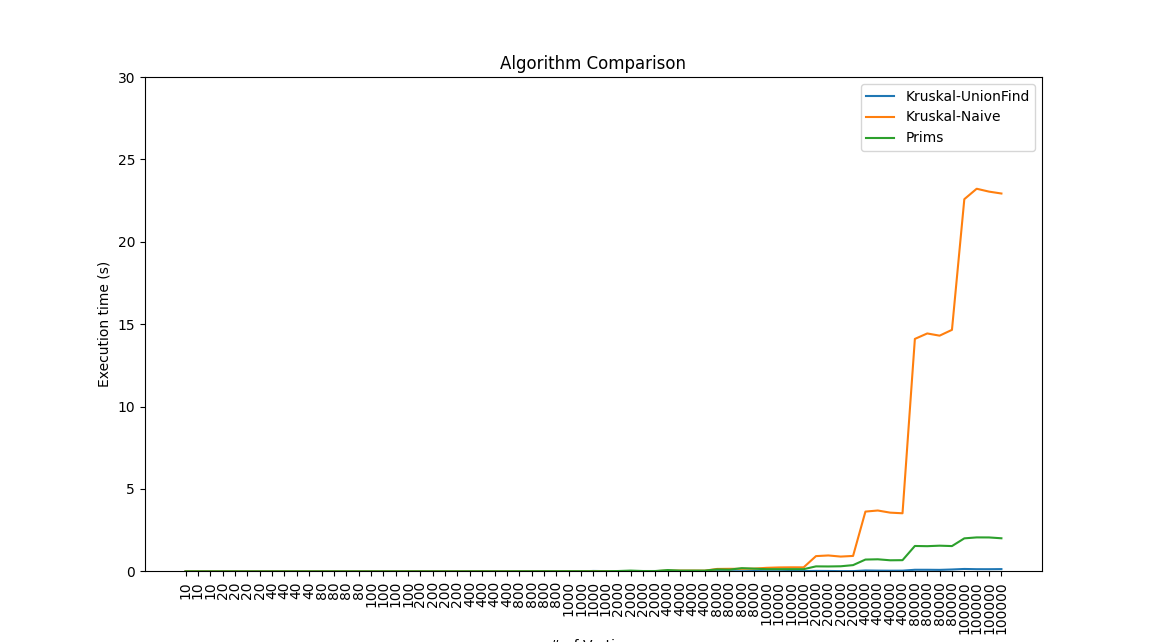
\includegraphics[width=19cm]{Img/AlgorithmComparison_Graph.png}
	\caption{Comparison between the performances of the three algorithms }
	\label{comparison}
\end{figure}

From Fig.~\ref{comparison} we can observe that for graphs with $1000$ vertices or less the performance are more or less the same.
When the number of vertices grows, the execution time of the Kruskal's ''naive'' algorithm grows exponentially and it could even take some minutes to calculate the MST of the bigger graphs of the dataset.
The execution time of Prim's and Kruskal's Union Find are very similar.
They take a few seconds to calculate the MST of the bigger graphs of the dataset. 
The results are consistent with the complexity of the algorithms.
Kruskal's ''naive'' is the most complex algorithm, instead the other two have the same algorithmic complexity but the Kruskal's Union Find has an execution time lower than Prim's.


\pagebreak